\documentclass[tikz,border=3pt]{standalone}
\usepackage[T1]{fontenc}
\usepackage{mathptmx}
\usepackage{pgfplots}
\pgfplotsset{compat=1.18}
\pdfinfoomitdate=1
\pdftrailerid{}
\pdfsuppressptexinfo=-1
\pgfplotsset{briefaxis/.style={
font=\fontsize{9}{11}\selectfont, tick label style={text=black},
label style={text=black}, title style={text=black},
axis line style={black,line width=0.6pt}, tick style={black},
axis background/.style={fill=white}, grid style={black!12},
legend style={text=black,font=\fontsize{9}{11}\selectfont,draw=none,fill=white},
unbounded coords=discard}}
\definecolor{briefblue}{HTML}{0072B2}
\definecolor{brieforange}{HTML}{D55E00}
\definecolor{briefgreen}{HTML}{009E73}
\begin{document}
% data_sha256=6cd6cc7034c8e26c51ccf8a717a2d70c1ce2f948e8073ff321c12561dce4c2db
\pgfplotsset{briefaxis/.style={
font=\fontsize{9}{11}\selectfont, tick label style={text=black},
label style={text=black}, title style={text=black},
axis line style={black,line width=0.6pt}, tick style={black},
axis background/.style={fill=white}, grid style={black!12},
legend style={text=black,font=\fontsize{9}{11}\selectfont,draw=none,fill=white},
unbounded coords=discard}}
\definecolor{briefblue}{HTML}{0072B2}
\definecolor{brieforange}{HTML}{D55E00}
\definecolor{briefgreen}{HTML}{009E73}

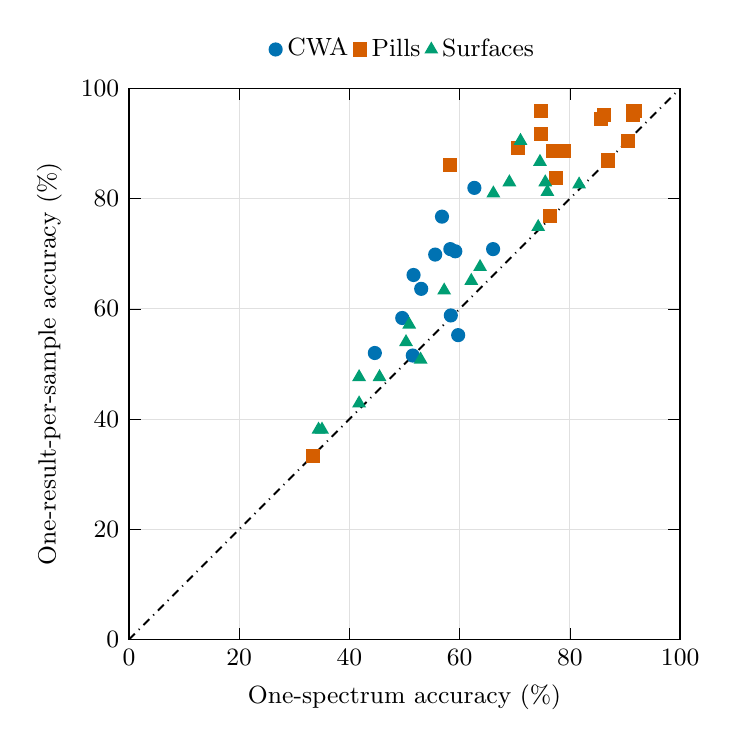
\begin{tikzpicture}
\begin{axis}[briefaxis,width=7cm,height=7cm,scale only axis,xmin=0,xmax=100,ymin=0,ymax=100,
xtick={0,20,40,60,80,100},ytick={0,20,40,60,80,100},grid=major,
xlabel={One-spectrum accuracy (\%)},ylabel={One-result-per-sample accuracy (\%)},
legend style={at={(0.5,1.03)},anchor=south,legend columns=3}]
\addplot[black,dash dot,line width=0.7pt,forget plot] coordinates {(0,0)(100,100)};
\addplot[only marks,mark=*,mark size=2.2pt,color=briefblue,line width=0.7pt] coordinates {(59.2063492063,70.4365079365) (53.0158730159,63.6243386243) (56.7857142857,76.7195767196) (55.5555555556,69.8412698413) (51.6269841270,66.1375661376) (44.6031746032,51.9841269841) (51.4920634921,51.5211640212) (58.3915343915,58.7962962963) (59.7248677249,55.2248677249) (58.3030303030,70.8333333333) (62.6666666667,81.9444444444) (66.0606060606,70.8333333333) (49.5757575758,58.3333333333)};
\addlegendentry{CWA}
\addplot[only marks,mark=square*,mark size=2.2pt,color=brieforange,line width=0.7pt] coordinates {(58.1818181818,86.1111111111) (74.7727272727,91.6666666667) (85.6060606061,94.4444444444) (70.6060606061,89.1666666667) (74.7727272727,95.8333333333) (91.3752913753,95.8333333333) (86.2470862471,95.2380952381) (76.4568764569,76.7857142857) (91.3752913753,95.2380952381) (91.8414918415,95.8333333333) (33.3333333333,33.3333333333) (33.3333333333,33.3333333333) (33.3333333333,33.3333333333) (33.3333333333,33.3333333333) (33.3333333333,33.3333333333) (76.8849206349,88.5714285714) (77.4140211640,83.8095238095) (77.4140211640,88.5714285714) (79.0013227513,88.5714285714) (77.4140211640,83.8095238095) (86.9047619048,86.9047619048) (86.9047619048,86.9047619048) (86.9047619048,86.9047619048) (86.9047619048,86.9047619048) (90.4761904762,90.4761904762)};
\addlegendentry{Pills}
\addplot[only marks,mark=triangle*,mark size=2.2pt,color=briefgreen,line width=0.7pt] coordinates {(50.2645502646,53.9682539683) (52.9100529101,50.7936507937) (34.3915343915,38.0952380952) (45.4545454545,47.6190476190) (41.7508417508,42.8571428571) (35.0168350168,38.0952380952) (41.7508417508,47.6190476190) (50.8417508418,57.1428571429) (75.9090909091,81.2121212121) (74.2424242424,74.8484848485) (81.6666666667,82.5757575758) (66.1111111111,80.9523809524) (71.0317460317,90.4761904762) (62.1031746032,65.0793650794) (74.5689655172,86.6666666667) (69.0134099617,82.9629629630) (75.5268199234,82.9629629630) (57.1839080460,63.3333333333) (63.6973180077,67.5925925926)};
\addlegendentry{Surfaces}
\end{axis}
\end{tikzpicture}\end{document}
